\documentclass[11pt,a4paper]{article}

% --- Paquetes ---
\usepackage[utf8]{inputenc}
\usepackage[spanish,es-tabla]{babel}
\usepackage[margin=2.5cm]{geometry}
\usepackage{amsmath,amssymb}
\usepackage{graphicx}
\usepackage{xcolor}
\usepackage{hyperref}
\usepackage{booktabs}
\usepackage{enumitem}
\usepackage{microtype}
\usepackage{titlesec}
\usepackage{fancyhdr}

% --- Configuración de hipervínculos ---
\hypersetup{
    colorlinks=true,
    linkcolor=blue!70!black,
    citecolor=blue!70!black,
    urlcolor=blue!70!black
}

% --- Encabezado y pie de página ---
\pagestyle{fancy}
\fancyhf{}
\lhead{\small Computación Paralela y Distribuida -- 2026-2}
\rhead{\small Tarea No. 02}
\cfoot{\thepage}

% --- Título e información ---
\title{\textbf{Universidad Nacional de Colombia}\\[0.3em]
\Large \textbf{Computación Paralela y Distribuida}\\
\large \textbf{Tarea No. 02: Capítulo 2 -- Patrones de Paralelismo}}
\author{\textbf{Jonathan López}}
\date{}

\begin{document}

\maketitle


\vspace{1em}
\hrule
\vspace{1.5em}

% =========================================================================
% PUNTO 1
% =========================================================================
\section{El texto utiliza los siguientes símbolos, entre otros, para representar los componentes fundamentales de los algoritmos. Para cada símbolo, describir de manera breve en qué momento se utiliza:}

\begin{center}
    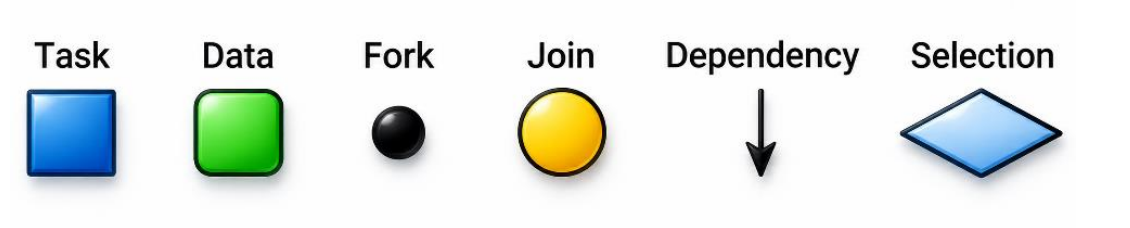
\includegraphics[width=0.5\textwidth]{Iconos.png}
\end{center}
\begin{itemize}[leftmargin=2em, itemsep=0.8em]
    \item \textbf{Task (Tarea):}

    Se utiliza cuando se opera sobre los datos, entran datos (inputs) y salen datos (outputs). Se representa con un rectángulo azul.
    \item \textbf{Data (Datos):}

    Se utiliza cuando se necesita representar la información, tanto de entrada como de salida de una tarea. Se representa con un rectángulo redondeado verde.

    \item \textbf{Fork (Bifurcación / División):}

    Se utiliza cuando se divide un flujo serial en varios flujos seriales creando paralelismo. Se representa con un punto negro.

    \item \textbf{Join (Unión / Sincronización):}

    Se utiliza cuando se necesitan unir varios flujos seriales separados en un solo flujo. Se representa con un punto amarillo.

    \item \textbf{Dependency (Dependencia):}

    Se usa cuando hay una dependencia temporal entre un par de tareas, puede ser una dependencia de datos o una dependencia de control. Se representa con una flecha.

    \item \textbf{Selection (Selección):}

    Aunque no se muestra en el capítulo dos, se usa cuando el algoritmo toma alguna decisión en un flujo de control. Se representa con un rombo azul claro.

\end{itemize}

\vspace{1.5em}

% =========================================================================
% PUNTO 2
% =========================================================================
\section{Responder las siguientes preguntas con base en el texto:}

\begin{enumerate}[label=\textbf{\alph*)}, leftmargin=2em, itemsep=1em]
    \item \textbf{¿Qué es paralelismo en datos?}
    El paralelismo en datos en el texto se define como cualquier tipo de paralelismo que crece a medida que la cantidad de datos crece.

    \item \textbf{¿Qué es descomposición funcional?}
    Es el opuesto al paralelismo en datos, en el que se corren diferentes funciones de un programa en paralelo.

    \item \textbf{¿Cuál es la relación entre el paralelismo en datos y la descomposición funcional?}
    Son estrategias opuestas con capacidades de escalabilidad diferentes, mientras que el paralelismo en datos consigue un paralelismo escalable, en la descomposición funcional se logra una mejora de rendimiento de un factor constante.

\end{enumerate}

\vspace{1.5em}

% =========================================================================
% PUNTO 3
% =========================================================================
\section{Los autores del libro consideran ambiguo el término de paralelismo basado en tareas (\textit{task parallelism}) y consideran más útil una clasificación basada en el "grado de regularidad". ¿Cuáles son los términos propuestos por ellos para esta clasificación? y ¿qué características tienen las tareas que incluye cada término?}


Los términos propuestos son:
\begin{itemize}[leftmargin=2em, itemsep=0.8em]
    \item \textbf{Paralelismo Regular:} Las tareas son similares y son predecibles las dependencias entre ellas.

    \item \textbf{Paralelismo Irregular:} Las tareas no son similares y crean dependencias impredecibles entre ellas.
\vspace{1.5em}
\end{itemize}

% =========================================================================
% PUNTO 4
% =========================================================================
\section{El concepto de tarea visto en clase con la analogía de arbustos de café ¿Es el mismo concepto que describe el siguiente párrafo? En la analogía de arbustos de café ¿Qué concepto sería el análogo al hilo mencionado aquí?}


\begin{quote}
\small
\textit{``We use task to refer to a unit of potentially parallel work with a separate flow of control. Tasks are executed by scheduling them onto software threads, which in turn the OS schedules onto hardware threads. A single software thread may run many tasks, though it actively runs only one task at a time. Scheduling of software threads onto hardware threads is usually preemptive---it can happen at any time. In contrast, scheduling of tasks onto software threads is typically non-preemptive (cooperative)---a thread switches tasks only at predictable switch points. Non-preemptive scheduling enables significantly lower overhead and stronger reasoning about space and time requirements than threads. Hence, tasks are preferable to software threads as an abstraction for scalable parallelism.''}
\end{quote}

\noindent\textbf{Nota de traducción técnica:}
\begin{itemize}[itemsep=0.2em]
    \item \textit{Scheduling:} Planificación [planificar]
    \item \textit{Preemptive:} Con derecho preferencial
    \item \textit{Non-preemptive:} Sin derecho preferencial (cooperativo)
\end{itemize}

\vspace{0.8em}
\noindent\textbf{Respuesta:}
Sí, en el texto una tarea es una unidad de trabajo potencialmente paralelizable con un flujo de control separado; en la analogía, un arbusto de café representa una unidad de trabajo separada que puede ser paralelizable por los recolectores. En la analogía del café, un hilo sería un plan de recolección, algo como una lista de arbustos a recolectar.


\vspace{1.5em}

% =========================================================================
% PUNTO 5
% =========================================================================
\section{Punto 5: Taxonomía de Flynn}



\noindent\textit{Con base en la subsección 2.4.3 y \url{https://en.wikipedia.org/wiki/Flynn's_taxonomy}, describa brevemente las cuatro categorías de paralelismo de Flynn.}
\begin{center}
    \includegraphics[width=0.5\textwidth]{Flynn.png}
\end{center}

\begin{enumerate}[label=\textbf{\arabic*.}, leftmargin=2em, itemsep=1em]
    \item \textbf{SISD (\textit{Single Instruction, Single Data}):}
    Un computador secuencial que no usa paralelismo ni en los datos ni en las instrucciones, que ejecuta una instrucción a la vez sobre un solo flujo de datos. Es el modelo tradicional de computación.

    \item \textbf{SIMD (\textit{Single Instruction, Multiple Data}):}
    Una única operación es ejecutada al mismo tiempo sobre varios datos, también son llamados procesadores de arreglos.

    \item \textbf{MIMD (\textit{Multiple Instruction, Multiple Data}):}
    Múltiples flujos de operaciones con flujos de control separados operan sobre datos separados. Cuando se tienen diferentes procesadores con diferentes arquitecturas, se denomina computador heterogéneo.

    \item \textbf{MISD (\textit{Multiple Instruction, Single Data}):}
    No es muy útil o usado, múltiples instrucciones operan sobre un flujo de datos.
    

\end{enumerate}

\end{document}

